\chapter[Ifi 1]{Informatikkbygningen – veien fram til eget hus}

\label{chap:ifi1}

\author{Skrevet av Narve Trædal}

\begin{figure}[h!]
	\centering
	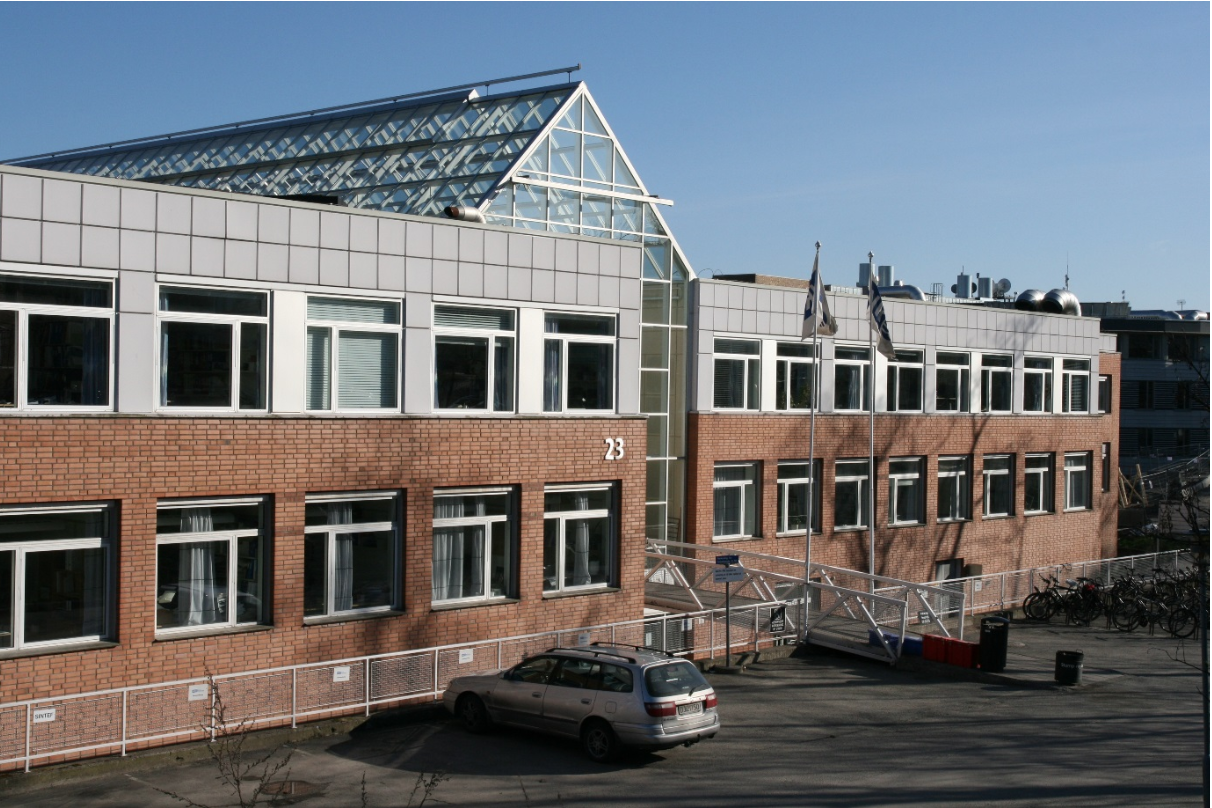
\includegraphics[width=0.8\textwidth]{images/ifi1/ifi1.png}
	\caption{Informatikkbygningen, som ble omdøpt til Kristen Nygaards hus da Ole-Johan Dahls hus sto ferdig i 2011.}
\end{figure}

Med tanke på lokale var situasjonen for det nye instituttet relativt kummerlig. I startfasen hadde instituttet lokaler i Matematikkbygningen: administrasjonen og faggruppen for kybernetikk, som var flyttet fra Fysikkbygningen, hadde lokaler i 5. etasje, mens databehandlere og numerikere stort sett beholdt sine gamle kontorer, og befant seg således marmorert inn i tre etasjer i Matematisk institutts arealer. I 1980 ble instituttet flyttet til Fysikk-bygningen, og fikk lokaler i østfløyen. Dette var et framskritt, sett fra et samlingssynspunkt, men heller ikke denne situasjonen var tilfredsstillende, selv om fysikerne la godviljen til. Mye tid gikk med til å løse akutte romproblemer, ofte på bekostning av Fysisk institutt.

\begin{wrapfigure}{r}{8cm}
\centering
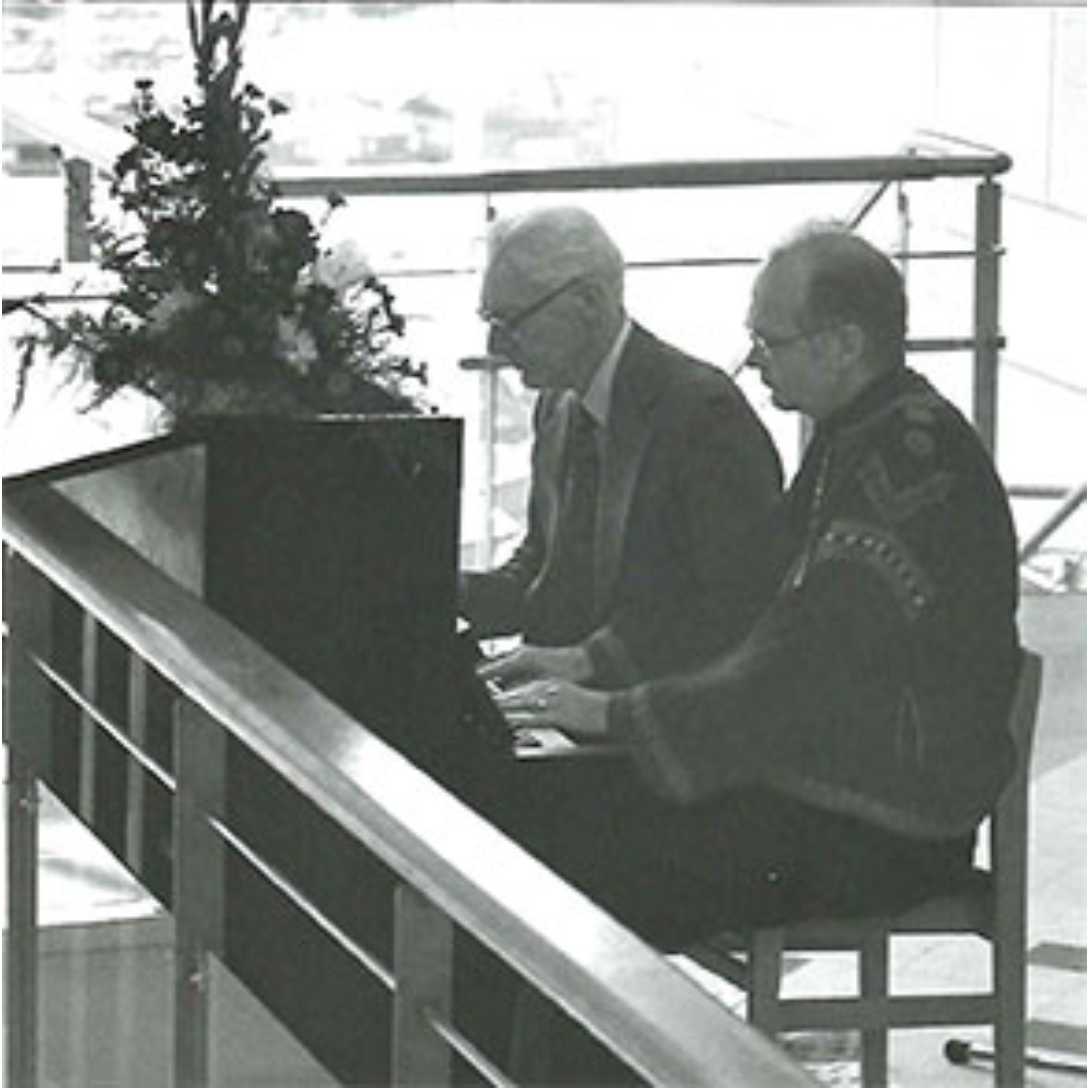
\includegraphics[width=0.6\textwidth]{images/ifi1/piano-ojd-og-donald-knuth.png}
	\caption{Donald Knuth og Ole-Johan Dahl i aksjon under åpningen av Informatikkbygningen. Knuth var verdensberømt professor ved Stanford University, og ble utnevnt til æresdoktor ved UiO i 2002.}
\end{wrapfigure}

I begynnelsen av 80-årene dukket idéen om et eget informatikkbygg opp. En sentral person også i dette arbeidet var ``instituttgründeren'' Arne Jonassen, som nå hadde permisjon og var ansatt som assisterende direktør i Norsk Regnesentral. Han fikk bygningen inn i NRs budsjettforslag for 1980, og misjonerte for en samlokalisering av informatikkmiljøene på Blindern, for Ifi og Universitetets sentrale EDB-tjeneste, USE, som EDB-senteret nå var omdøpt til. Til Jonassens egen forbauselse skjedde ting med rekordfart. ``Det var sannsynligvis noen flere aktører parallelt, som sparket ballen opp i førstedivisjon'', forteller han i et intervju. Blant disse parallelle aktørene var blant annet Lars Walløe, som var instituttbestyrer ved Ifi i perioden 1980-88. Han arbeidet tett sammen med rektor ved UiO, Bjarne Waaler, og NTNF-direktør Gudmund Harlem. Sammen laget de en samlet løsning, så å si over bordet. UiO hadde ingen penger, men opsjon på en tomt i Gaustadbekkdalen som opprinnelig var tenkt til nytt universitetsbibliotek. NTNF hadde penger, men ingen tomt, og UiO forpliktet seg så til en langsiktig leieavtale.

Sjelden har en byggeprosess forløpt smidigere. Da Arne Jonassen kom tilbake til Ifi i 1982, ble han valgt inn i byggekomitéen som straks satte i gang med å fordele plass og rom til institusjonene som skulle inn. Selv om Ifi så at også dette husrommet ville bli trangt, så innså man at dette var det beste man kunne håpe på.

Byggearbeidene gikk ellers problemfritt, og Ifi og NR flyttet inn sommeren 1988. Selv om det også i det nye huset relativt fort meldte seg ombyggingsbehov, og kapasiteten var sprengt nærmest før innflytting, så var altså nå instituttet for første gang herre i `eget' hus. Den høytidelige åpningen fant sted 19. september samme år, med inviterte gjester, foredrag og kunstneriske innslag, blant annet firhendig pianospill av Donald E. Knuth og Ole-Johan Dahl. Gaustadbekkdalen ble av universitetsavisen UNIFORUM omdøpt til ``Datadalen''.

Men det ble som sagt trangt. NR holdt til i 4.etasje, USE og Ifi delte resten. USE, som ble omdøpt til USIT i 1991, etter at EDB-senteret og ADB-avdelingen formelt ble slått sammen, var på litt vikende front, og måtte flytte deler av virksomheten sin ut i en brakke som hadde vært brukt i forbindelse med byggingen av Forskningsparken, og som lå nord for Informatikkbygningen. Og få år etter tok også Ifi denne brakka i bruk. I 1995 disponerte Ifi 65 hovedfagsplasser, 2 seminarrom og en 1 terminalstue, pluss pause- og skriverrom, der. 

Brakka måtte bøte med livet i 2001 i forbindelse med byggingen av SINTEFs MiNALab, men det er en god del informatikere rundt om i landet som forbinder sin studietid, i alle fall på hovedfag, med en `brakketilværelse'. Forhåpentligvis er det likevel gode minner.
